\chapter{Pithos Design and Implementation}
\label{chp:DESIGN}

The generic state consistency model was presented in Section \ref{generic_event_update_model}. One of the key challenges that still remain was determined to be designing a root storage module specifically tailored to P2P MMVEs. The root storage model identifies in Section \ref{generic_event_update_model} includes the processes of state management and state persistency for the authoritative objects.

We've identified the main requirements of P2P MMVE state management and persistency in in Section \ref{key_challenges_cm} as: scalability,
reliability, fairness, responsiveness and security. In Chapter \ref{p2p_MMVE_state_persistency} it is argued that none of the current approaches to state persistency satisfy all identified requirements,

The focus of this thesis is, therefore exclusively on state management and persistency in P2P MMVEs. This chapter presents a design that satisfies all the identified requirements, along with implementation details and results.

Pithos, a novel hybrid multi-tiered state persistency architecture is
proposed. The novelty of Pithos lies in its support for both a responsive and a fair storage system, while also taking into account security aspects
of distributed storage. There are some storage systems that provide responsive or fair storage, but none that provide both. No storage system, designed specifically for P2P MMVEs, have taken security into account.

If Pithos is incorporated into an existing P2P MMVE consistency architecture, it will add the ability to handle both state management and state persistency. The addition of a robust state persistency mechanism, specifically designed for P2P MMVEs, will bring us one step closer to
the creation of a complete P2P MMVE architecture.
%%%%%%%%%%%%%%%%%%%%%%%%%%%%%%%%%%%%%%%%%%%%%%%%%%%%%%%%%%%%%%%%%%%%%%%

\section{Use cases}

The purpose of Pithos is to allow for efficient object storage and retrieval that satisfies all identified requirements. As is evident from root storage in the flow diagram in Figure \ref{fig_event_update_flowdiagram}, Pithos will interface directly with the VE logic, as well as receive updates from the update generator. For the purposes of this discussion, update generation is assumed to be part of game logic.

\begin{figure}[htbp]
 \centering
 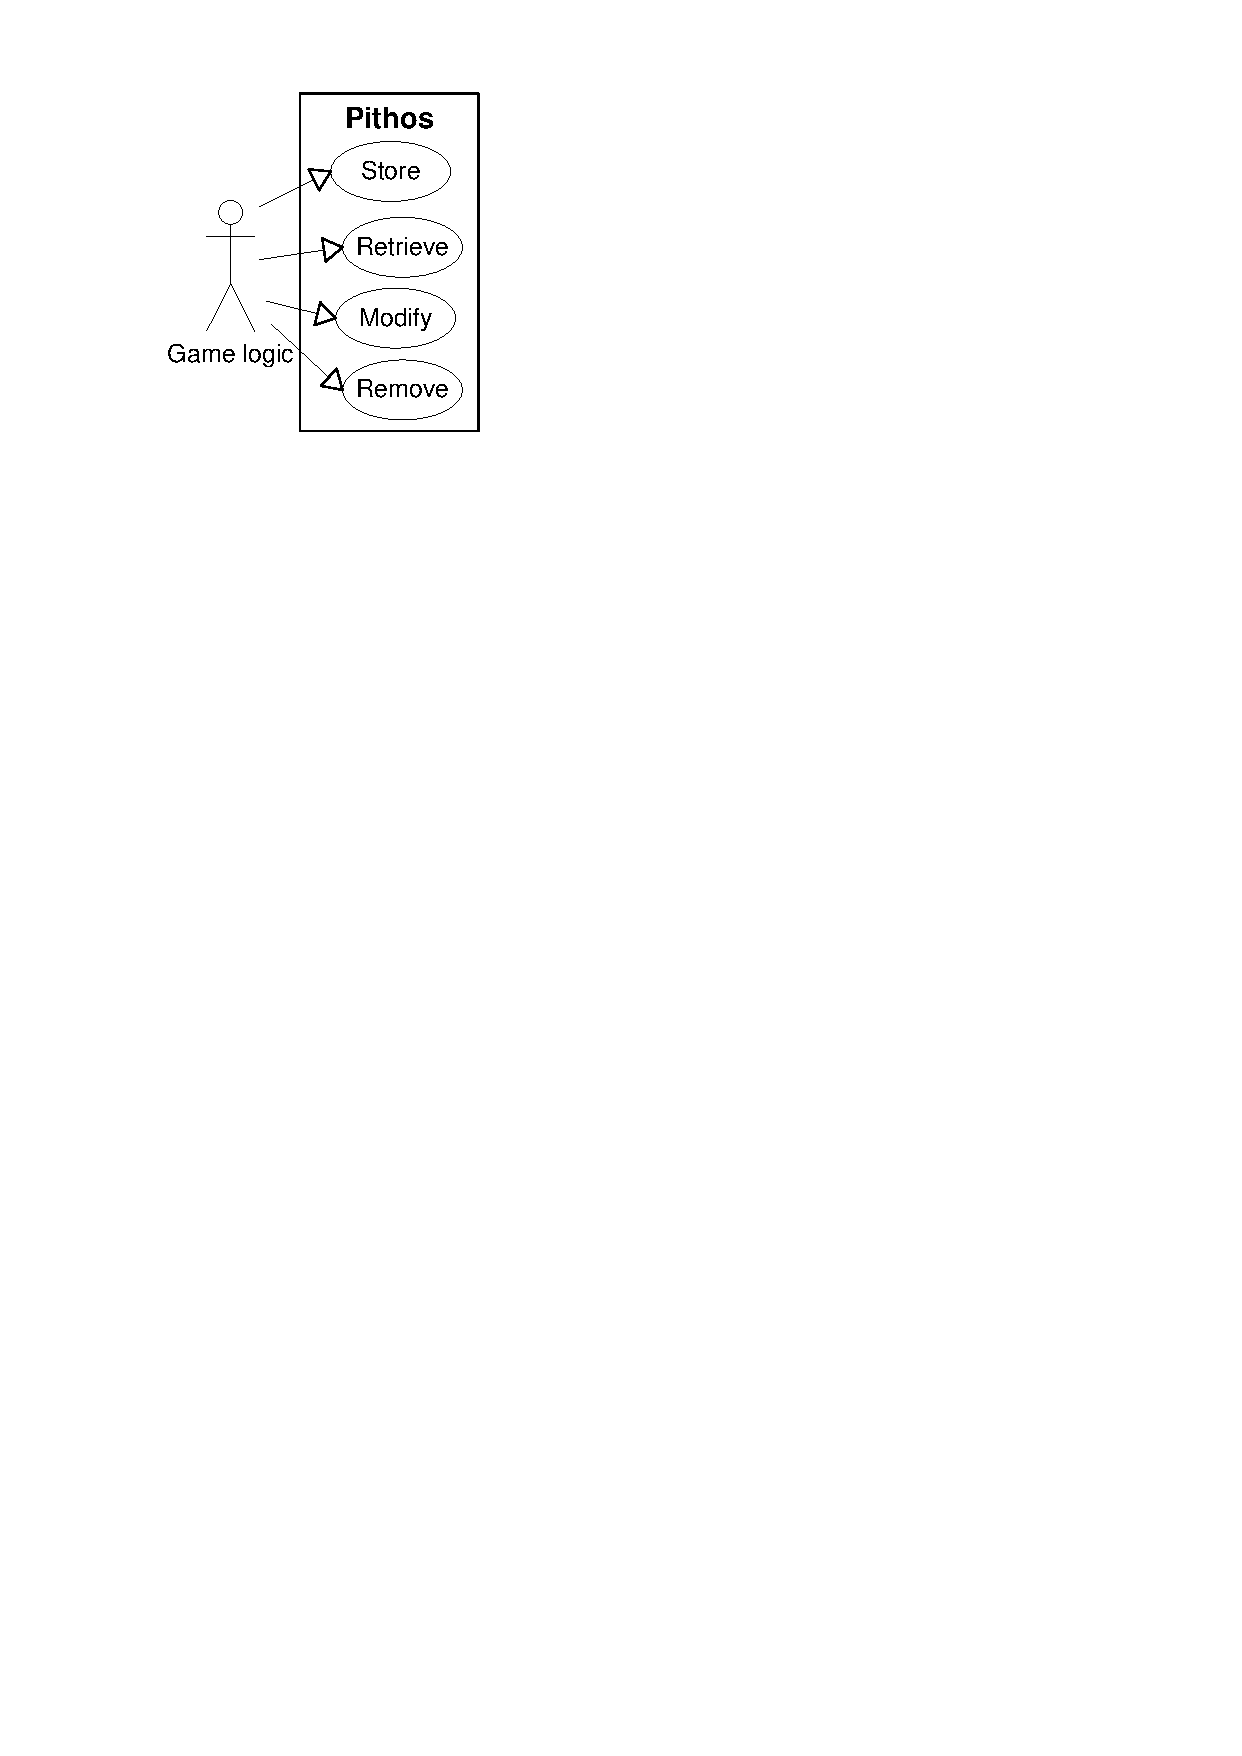
\includegraphics[clip=true, viewport=28mm 223mm 82mm 282mm, width=0.5\textwidth]{pithos_use_case}
 \caption{Use case diagram of Pithos}
 \label{fig_pithos_use_case}
\end{figure}

As shown in the use case diagram in Figure \ref{fig_pithos_use_case}, the VE logic should be able to use Pithos in four ways: store, retrieve, modify and remove. These are the use cases generally required of any storage system.

The VE logic will store data when a new object is added to the VE state. This can happen as a consequence of an event leading to the generation of a new object. An example of this is a rocket firing at a target. This event might generate a missile object to be sent towards the target.

Object retrieval will be required every time an event is received. The VE logic will retrieve the object state from memory, which is part of state management. Object states, other than the one being altered, might also be required by the logic to determine the effect an event will have, as discussed in Section \ref{event_logic_update}.

Object modification occurs every time an object update is generated. An object update, by definition, required a modification of the object state.

Object removal might also be required to save storage space, although this is not essential to the correct functioning of the storage system.

\section{Design goals}

\section{Architecture characteristics}

In this section, ``Pithos'', the proposed P2P MMVE state persistency architecture design is described. The inspiration for this architecture come
from two observations:
%
\begin{enumerate}
  \item One can combine multiple storage models and arrive at a model which possesses fewer disadvantages than any of the models used.
  \item Responsiveness is greatly increased in a fully distributed model, where there is no intermediate server that relays all information.
      However, fully distributed architectures are not scalable because the number of messages scaling by $O(N^2)$, where $N$ is the number of
      nodes in the network.
\end{enumerate}

\begin{figure}[htbp]
 \centering
 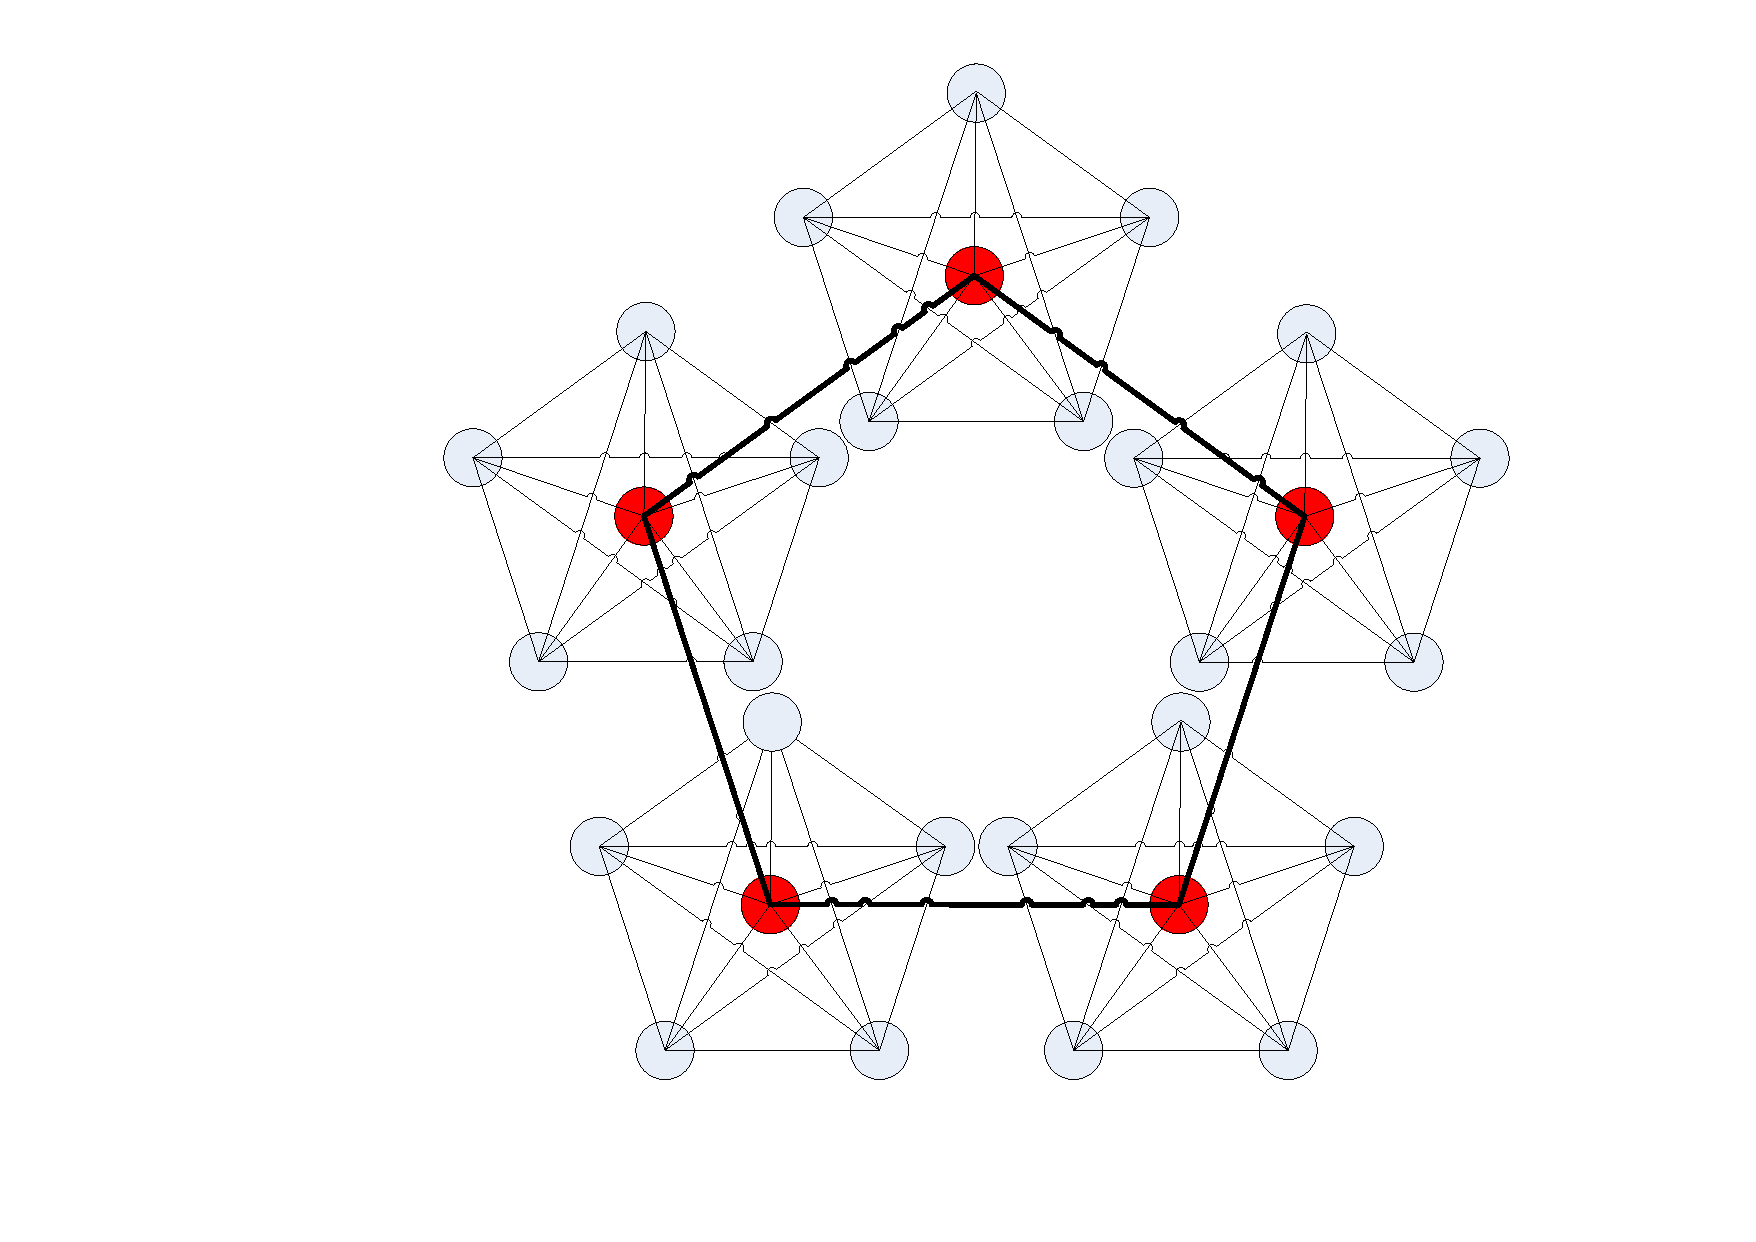
\includegraphics[clip=true, viewport=7.5cm 2.5cm 26cm 20cm, width=0.7\columnwidth]{CDHT_layout}
 \caption{Layout of the Pithos storage architecture}
 \label{fig_pithos}
\end{figure}
%
Figure \ref{fig_pithos} shows the Pithos architecture. The figure shows groups of fully connected peers (light blue and dark red), where all groups
are connected to each other in an P2P overlay through super peers (red).

Pithos groups peers to form a two tiered storage model. The first tier is a storage model at group level and the second is a storage model over all
groups. On the first tier, which is the intra-group level, a fully distributed storage system is used to allow for highly responsive read and write
operations within the group. On the second tier, which is the inter-group level, a P2P overlay is used to store data between groups.

According to categorisation of \ref{storage_type_overview}, Pithos is a type of hybrid storage, that incorporates overlay storage and distance-based
storage. Responsiveness is achieved by constructing fully connected networks amongst groups of players and then storing objects that are mostly used
by the group within the group, as described in Sections \ref{grouping}, \ref{store_retrieve} and \ref{distance_based}. Reliability is achieved by
making use of replication and migration mechanisms as described in Section \ref{store_retrieve}. Security is achieved by using a certification
authority to assign node IDs and signing any storage and retrieve request with the requesting node's certificate, as described in Section
\ref{secure_ids}. Fairness is achieved by having all nodes store objects, as described in Sections \ref{store_retrieve} and \ref{distance_based}.

\subsection{Grouping}
\label{grouping}

%Speak more concretely of grouping algorithms
At the core of the architecture is the peer clustering mechanism. Two approaches are being evaluated: distributed clustering techniques (for example
affinity propagation \cite{affinity_propagation}) and dynamic regioning techniques (for example self-organising spatial publish subscribe (SOSPS)
\cite{self_organising_sps_post}).

\emph{Distributed peer clustering techniques}: make use of the flocking behaviour of players to dynamically group players into flocks or clusters
\cite{flocking}. The main idea of flocking is that players move around in groups, rather than randomly on their own. It is desirable that user
density within groups should remain constant, because a fully distributed architecture is not scalable. This means that groups should merge or split
as the user density within them change.

Affinity propagation clusters nodes using a similarity matrix to find similar nodes. The similarity matrix may contain user positions. In this case,
affinity propagation will group nodes depending on their location in a virtual world. This algorithm is ideally suited to P2P applications, since it
is a distributed clustering algorithm based on message passing.

\emph{Dynamic regioning}: divides the virtual world into regions that can be resized or further divided to maintain constant player densities across
regions. SOSPS creates dynamic regions based on a Voronoi overlay network \cite{voronoi_diagrams_survey}. Near constant user density is achieved by
increasing and decreasing the area sizes. This system is based on VON, a distributed Voronoi overlay network designed for MMVEs \cite{VON_VAST}.

\subsection{Replication}
\label{store_retrieve}

When storing objects in Pithos, replication is used to increase object availability under network churn and for security in the presence of malicious
nodes \cite{storage_and_chaching_PAST}. For every object that is stored in Pithos, $k$ object replicas are also stored. The number of replicas ($k$)
depends on the degree of network churn as well as the number of expected malicious users in the network. If the network churn is high, more replicas
are required to avoid the situation where all $k$ peers hosting an object leaves the network before any object migration can be done.

If a node leaves the network and stops to transmit ``keep alive'' messages, the migration mechanism will detect this and replicate the file on
another node. Replication exists intra- as well as inter-group and is useful in ensuring that if a nodes leaves the network, the data are not lost.
All object requests are routed to the peer with the next closest ID if the root peer leaves, because of how overly routing functions. The new
destination peers will possess the stored files, since Pithos stores overlay replicas at overlay neighbours.

Another reason to replicate game objects is to make the system more secure. If it is known that a certain percentage of users are malicious, it is
advantages to have more replicas than malicious users. This will allow for a secure system where object hashes can be compared to determine which
nodes are malicious and what version of an object is accurate.

\subsection{Distance-based storage}
\label{distance_based}

For Pithos to succeed as an MMVE storage architecture, intra-group data requests should be preferred to inter-group data requests. This requirement,
combined with the fact that the grouping algorithm geographically groups players in the virtual world, lends Pithos to a storage system based on
distance-based storage. Similar to interest management, the assumption is that players have a limited area of interest and require interaction with a
limited number of objects within range.

Therefore, distance-based storage is implemented on a group level rather than an individual level. This means that objects are stored on the nearest
group of players, rather than the nearest user. It is assumed that such an approach will alleviate the security and reliability challenges present in
distance-based storage \cite{gilmore_p2p_mmog_state_persistency}.

With group-based distance-based storage, it is assumed that because peers now store objects closest to the group, the objects that they are
interested in will most likely be stored within their own group. Therefore, most data requests should be intra-group requests. The overlay storage
component ensures that nodes that require data, which are not stored within their group, are still able to access requested data.

\subsection{Secure storage and node ID assignments}
\label{secure_ids}

In order to design a secure distributed storage system, one requirement for the P2P overlay is that nodes should not be able to select their own IDs
or it will not be possible to secure the system against attack. Node IDs should rather be assigned securely by some certification authority
\cite{secure_overlay_routing}.

To meet this requirement, Pithos implements its own certification authority to assign node IDs securely and promote security in the P2P overlay. A
certification server exists that handle ID requests from nodes. The server assigns IDs to nodes and provides the node with a signed certificate that
it may use to store data.

Whenever an object is stored or updated in the storage network, nodes have to sign the object to enable the tracking of object changes throughout the
life of the object. This system is very different from classic distributed file storage designs that advocate anonymity in storage. The fact that all
changes can be tracked to a specific node will simplify the task of eliminating user cheating.

\section{Implementation details}

\subsection{Oversim architecture}
    \subsection{Structure}

        \subsection{DHT implementation}

    \section{Data structures}

        \subsection{Game object}

        \subsection{Group ledger}

    \section{Joining the network}

    \section{Storing data}

    \section{Retrieving data}

    \section{Modifying data}

    \section{Designing for network churn}

    \section{Group consistency}
    %Check how this increases with increased network sizes and varying levels of network churn.

    \section{Repair mechanisms}

    \section{Group migration}
    
        \section{Bandwidth requirements (overhead)}
    %Mention something about low bandwidth links and how that influences timeout and what extra mechanisms were required.
    %Check how this increases with increased network sizes and varying levels of network churn.

    \section{Implementation}
    The proposed multi-tiered model is currently being implemented in Oversim \cite{OverSim_2007}, a P2P simulation environment based in Omnet++, which
allows for the measurement of identified requirements. Furthermore, it allows for the comparison of the current model with other state persistency
models. Initial results are promising, with the implemented model functioning as expected. The simulated system is very responsive when storing data
within a group and as responsive as storing data in an overlay, when storing data between groups.

Pithos is designed to form part of a complete P2P MMVE network solution. It is assumed that there exists some intelligence that drives Pithos and has
to determine when objects have to be stored and retrieved on each peer. This driving intelligence is termed the game layer.

In the results shown, Pastry was used as the P2P overlay and Pithos was driven by a \emph{Game} module developed for this purpose. After a node has
joined a group, the game module starts to generate store and retrieve requests at a rate of 10 objects per second and a size of 1024 bytes. The size
of 1024 byte objects was chosen to be much larger than Quake 3 game objects without delta encoding, used in \cite{Bharambe_Donnybrook}. Pithos is
designed for the low latency storage of small game objects.

For the results shown, 14499 peers, 500 super peers and a single directory server are created at the start of the simulation. The directory server
publishes super peer information, which allows a peer to join the group nearest to it. Because of the way Pithos is structured, each super peer node
is also a peer node, which gives a total of 15000 Oversim nodes.

To be able to simulate Pithos for 15000 nodes, it runs on the Oversim simple underlay network \cite{oversim_applications}, where node latencies are
determined by the distance between nodes placed in an $n$-dimensional Euclidean space. The positions of the nodes are chosen to match the latencies
of the CAIDA/Skitter project. Different nodes are also assigned different bandwidth and jitter parameters to simulate a heterogenous network.
